%% Materiales, imprsion 3D

\chapter[Marco Te\'orico.]{Marco Te\'orico}
%-------------------------------------------------------------------------------------
% [RR] En este cap quiero iniciar con empezar hablando un poco de lo que es calidad del agua, hablar sobre los factores físico - químicos quede deben de tenerse en cuenta, profundizar los paráme tros físicos químicos que yo utilizo (temp, ph, conductividad eléctrica, opr, salinidad, total solidos disueltos, oxigeno disuelto.  .
% [RR]Luego quiero profundizar en cada sección:
% [RR]-> un poco sobre cada uno de los sensores, tipo, funcionamiento, 
% [RR]-> Tipos de muestreos manuales y automáticos, opciones comerciales, (énfasis al valor agregado de medicion a multinivel)

\section{Monitoreo de Agua.}
El agua es un recurso presente en la naturaleza, indispensable para la vida misma e infiere en la mayoría de los procesos industriales \cite{estudio_agua}, en el planeta el 2.5 \% del agua es dulce, de los cuales el 69 \% se encuentra en estado sólido en los polos y cumbres de la monta\~nas altas del alrededor del mundo. El 30 \% del agua dulce del mundial, se encuentra en la humedad del suelo y en los acuíferos profundos, el 1 \% del agua dulce en el mundo se encuentran por las cuencas hidrográficas en forma de arroyos y ríos y se depositan en lagos, lagunas, acuíferos y en otros cuerpos superficiales de agua,  \cite{junta-municipal-de-agua-potable-y-alcantarillado-de-mazatlan-no-date}.
Un alto porcentaje de los recursos h\'idricos alrededor del mundo están contaminados por diversas causas, haciendo que estos ecosistemas el cual conforman se dañen gravemente y en el caso de no tomar las medidas de mitigación a tiempo, es posible que los da\~nos se tornen irreversibles, alterando gravemente al medio ambiente que a su vez un sin fin de problemas relacionados como perdida de fauna, flora y paisaje, enfermedades a las poblaciones aledañas además de todo el impacto económico y social que conlleva.
En la tabla \ref{tabla:analisisAgua} se pueden ver un an\'alisis realizado por S.Duenas, en Paraguay, uno de los problemas que se viene generando por la mala utilización de las tecnologías en la perforación de pozos en algunas zonas, y el que los graves problemas de contaminación en lugares lejanos de Brasil y Argentina, debido a la dinámica del agua, afectan la totalidad de la región,
\cite{salas-duenas-2015}.
\begin{table}[ht]
\caption{An\'alisis de la problemática del agua en paraguay}
\begin{tabular}{lll}
\hline
\multicolumn{1}{c}{\textbf{Actividad}}                                     & \multicolumn{1}{c}{\textbf{Efectos}}                                                                 & \multicolumn{1}{c}{\textbf{Área}}                                                                        \\ \hline\\
Urbana e industrial                                                        & \begin{tabular}[c]{@{}l@{}}Contam. superficial y  \\ acu\'iferos.\end{tabular}                 & \begin{tabular}[c]{@{}l@{}}REMA$^{\ast
}$\\ Cuenca de Ypacarai.\end{tabular} \\ \\
Mataderos,\\ frigor\'ificos                                                   & Aguas superficiales                                                                                  & REMA                                                                                                     \\ \\
\begin{tabular}[c]{@{}l@{}}EUD $^{\ast \ast}$ \end{tabular} & Destrucci\'on de \\                                                                       & \begin{tabular}[c]{@{}l@{}}Cuenca Ypacarai\\ Cuenca del Ypoa\end{tabular}                                                     
& REMA                                                                                                     \\ \\
\begin{tabular}[c]{@{}l@{}}Cementera\\ Metal\'urgica\end{tabular}            & \begin{tabular}[c]{@{}l@{}}Contaminaci\'on superficial \\ y acu\'iferos\end{tabular}                  & \begin{tabular}[c]{@{}l@{}}REMA\\ Villa Hayes\end{tabular}                                               \\ \\
Prácticas agrícolas.                                                      & \begin{tabular}[c]{@{}l@{}}Colmataci\'on por erosi\'on \\ y  pesticidas\end{tabular} & Todos los Dptos                                                                                          \\ \\ \hline
\end{tabular}
\bigskip

\small \textit{Nota}.$^{\ast}$ Regi\'on Metropolitana de Asunci\'on. \\$^{\ast \ast}$Expansi\'on Urbana desordenada. \textit{Fuente}:Adaptado,\cite{salas-duenas-2015}.
\label{tabla:analisisAgua}
\end{table}

En el informe publicado por la Organizaci\'on de las Naciones Unidas (ONU) para la Alimentaci\'on y la Agricultura (FAO) indica, que existen registros y monitoreos de la calidad de las aguas, sea de forma privada, como por intervenciones del estado, pedidos de la SEAM, controles de Dirección General de Salud Ambiental (DIGESA), no obstante, esta informaci\'on (recopilada por la SEAM) no es sistematizada, ni estudiada como para hacer un diagn\'ostico de la calidad de las aguas a nivel nacional, \cite{FAO_2015}.
Conocer el estado real de los recursos h\'idricos se puede tornar una tarea bastante complicada, donde una cantidad de factores que pueden influir, desde la t\'ecnica del monitoreo, la ubicaci\'on de las sondas fijas en caso de monitoreo autom\'atico o en la recolecci\'on de material para an\'alisis posterior en el caso de muestreos manuales.
En el caso monitoreo manual, a efecto de este trabajo se considera son los que se realiza mediante la recolecc\'on de muestras biol\'ogica in situ, almacenamiento temporal y traslado a un laboratorio donde se realizan las lecturas mediante robustas y normalizadas metodolog\'ias de an\'alsis con sensores de alta calidad, fidelidad y certeza de calibraci\'on.
El monitoreo manual involucra un importante despliegue log\'istico, t\'ecnicos, especialistas, recipientes de recolecci\'on, entre otros factores que pueden elevar bastante los costos de las campa\~nas de monitoreo, sin considerar las limitaciones que se podr\'ian presentar con respecto a la inaccesibilidad geogr\'afica que se pueden presentar para llegar al lugar de muestreo y la cantidad de material que se podr\'ian recolectar por motivos de almacenamiento y peso del material biol\'ogico.   
Las sondas fijas utilizadas en el monitoreo no requieren de constantes despliegues log\'isticos, posteriores a su instalac\'on, pero si requiere de una inversi\'on m\'as considerable y peri\'odicos mantenimientos. 
Por su alto costo de instalación no es posible cubrir en su totalidad del recurso h\'idrico a ser analizado. 
El Paraguay es un pa\'is muy rico hidr\'ogicamente, por la cantidad de agua dulce en su territorio, la hidrología de Paraguay está formada por cascadas, ríos, lagos,  humedales. También cuenta con una importante reserva subterránea del acuífero guaraní, que se comparte con los países vecinos.

\textbf{Los Humedales del  Paraguay.}

El Paraguay posee una extensa \'area de ambientes h\'umedos, conocidos como pantanales, selvas de ribera, embalsados, esteros y otras tantas denominaciones que tienen en com\'un ser considerados humedales por la convenci\'on Ramsar, \cite{salas-duenas-2015}. A partir del 7 de octubre de 1995, entr\'o en vigor en Paraguay la convención Ramsar, la Convención sobre los Humedales es el tratado intergubernamental que ofrece el marco para la conservación y el uso racional de los humedales y sus recursos, tiene actualmente 6 sitios designados como Humedales de Importancia Internacional, con una superficie de 785,970 hectáreas,\cite{ramsarWEB}.
Paraguay posee 22 regiones de humedales, de las cuales 6 han sido reconocidos como sitios Ramsar. Aproximadamente el 25\% de supercie está cubierta por humedales permanentes que no solo actúan como reservorios de agua, sino también concentran una importante
riqueza de biodiversidad, lo que representa un \'area que puede variar entre los 100.000 $Km^2$ y los 150.000 $Km^2$, respectivamente, \cite{mereles1998humedales}.
Algunos de los humedales del Paraguay, hacen parte de El Pantanal, que es considerado el mayor humedal del mundo, con unos 140,000 $Km^2$ y cubre \'areas en Brasil, Bolivia, y Paraguay. Forma las nacientes del R\'io Paraguay, considerado uno de los m\'as importantes reservorios de agua para los pa\'ises de la regi\'on.
Es el mayor reservorio de plantas acu\'aticas del hemisferio occidental y contiene grandes concentraciones de peces y aves, lo que posiblemente le confiere el contener la mayor concentraci\'on de especies acu\'aticas del mundo, \cite{willink2000biological}.
Estos humedales se encuentran distribuidos en las dos regiones naturales del pa\'is. La Occidental o Chaco, donde existen extensas \'areas con suelos formados b\'asicamente por arcillas y limos, los cuales no permiten la filtraci\'on del agua, facilitando la formaci\'on de extensos pantanales,\cite{vera2000iniciativas}.
L. Fernández Reyes y D. Moura, en su trabajo sobre los humedales, consideran que los humedales del chaco paraguayo son producto de la interacci\'on de las aguas de desborde del R\'io Paraguay al este, las inundaciones provenientes del r\'io Pilcomayo al sureste y las lluvias ocurridas al este de la regi\'on,\cite{fernandez2005humedales}.

\textbf{Agua subterránea}

Paraguay cuenta con varios acu\'iferos, en la figura \ref{acuiferosPy} se pueden observar su distribuci\'on en el territorio Paraguayo, considerando su nivel de explotaci\'on y el volumen de agua con lo que cuenta, los m\'as importantes son,\cite{FAO_2015}:
\begin{itemize}
    \item Acu\'ifero Yrendá, se estima que el Pilcomayo contribuye con 860 millones de $m^{3}$, y la recarga total se estima en  2.46$km^{3}$.
    \item Acu\'ifero Pati\~no: ubicada en la zona central del pais, según el Balance Hídrico Integrado de 2005, al Pati\~no ingresan 175.8 millones de $m^{3}$ y se extraen 249 millones de $m^{3}$. 
    \item El Acu\'ifero Guaran\'i: es compartido con Brasil, Argentina y 
    Uruguay, tiene un área total de 1,150,000 $km^{2}$, con 150,000 
    $km^{2}$ de recarga natural, arrojando un volumen promedio de 160 
    $km^{3}$ a\~no en total. Corresponde a Paraguay 67,000 $km^{2}$, con 
    37.000 $km^{2}$ de recarga, y un volumen de 39 $km^{3}$a\~no. 
\end{itemize}
Se estima que el volumen de los tres acu\'iferos m\'as importantes del pa\'is rondar\'ian los 41,64 $km^{3}$, \cite{alvarez-2014}.
El sistema del Acuífero Guaraní, tienen una superficie total de aproximadamente 1,2 millones de $km^{2}$, de los cuales unos 71,700 $km^{2}$ corresponderían a territorio paraguayo y se estima que en total unas quince millones de personas viven en su área de influencia,\cite{salas-duenas-2015}.

\begin{figure}[ht]
    \caption {Acuíferos del Paraguay} 
    \centering
    \label{acuiferosPy}
    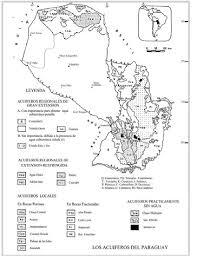
\includegraphics[scale=1]{Imagenes/cap2/images.jpg}\\
    \bigskip
    \raggedright
    \small \textit{Nota}. Extra\'ido de \cite{alvarez-2014} 
\end{figure}

Los principales usuarios del agua en el Paraguay son el consumo dom\'estico de la poblac\'on, la ganader\'ia, la agricultura con riego y la industria. 
Entre los usos no consuntivos se tienen las represas hidroel\'ectricas y la navegaci\'on que depende de los niveles del r\'io,\cite{groundwater_caracteristicas_2021}.
Hay una prevalencia del suministro de agua potable por medio de agua subterr\'anea, el 80$\%$ del abastecimiento de comunidades en el interior del pa\'is es con agua subterr\'anea. Esto genera una fuerte presi\'on sobre los acu\'iferos, con el consecuente peligro de contaminaci\'on que estos pozos representan, (en ocasiones construidos por el mismo Estado, sin cumplir los requerimientos t\'ecnicos y legales). El caso m\'as cr\'itico es el acu\'ifero Pati\~no, ubicado en la zona del departamento
Central con la mayor densidad demogr\'afica,\cite{alvarez-2014}.


\section{Legislaci\'on paraguaya}

El gobierno de Paraguay,trav\'es de su Direcci\'on General de Protecci\'on y Conservaci\'on de los Recursos H\'idricos (DGPCRH), protege los humedales y gestiona el manejo de los mismos con el fin de su conservaci\'on. Asimismo, la Direcci\'on General de Protecci\'on y Conservaci\'on de la Biodiversidad (DGPCB) es Punto Focal y autoridad de la Ley N$^{o}$ 350/94 \textit{"Que aprueba la Convenci\'on Relativa a los Humedales de Importancia Internacional, especialmente como h\'abitat de aves acu\'aticas”}, seg\'un lo establece la Ley N$^{o}$ 1561/00 \textit{"Que crea el Sistema Nacional del Ambiente, el Consejo Nacional del Ambiente y la Secretar\'ia del Ambiente"}, en inciso J. de su art\'iculo 14$^{o}$, \cite{direccion_general_de_proteccion_y_sitios_nodate}. 
Posteriormente, en la Ley N$^{o}$ 6.123/18 "\textit{Que eleva al rango de Ministerio a la Secretar\'ia del Ambiente y pasa a denominarse Ministerio del Ambiente y Desarrollo Sostenible (MADES)}, encargado del ordenamiento ecol\'ogico y del ambiente en general, propendiendo a un mejoramiento permanente de las condiciones de vida de los distintos sectores de la sociedad paraguaya para garantizar condiciones de crecimiento econ\'omico, equidad social y sustentabilidad ecol\'ogica a largo plazo. 
MADES es una entidad que tiene como funci\'on y prop\'osito formulaci\'on de pol\'iticas, la coordinaci\'on, la supervici\'on, la ejecuci\'on de las acciones ambientales, los planes, programas y proyectos enmarcados en el Plan Nacional de Desarrollo, referentes a la preservaci\'on, la conservaci\'on, la recomposici\'on y el manejo de los recursos naturales, \cite{mades_antecedentes_nodate}, constituye además  en autoridad de aplicación de la Ley N$^{o}$ 3,239/07 "De los Recursos Hídricos del Paraguay", \cite{noauthor_presidente_nodate}, que introduce el marco normativo para la gestión integral y sustentable de los recursos hídricos. 
Dicha gestión debe basarse en los principios enunciados por las presentes disposiciones, entre los cuales cabe destacar los siguientes: las aguas, superficiales y subterráneas, son propiedad de dominio público del Estado y su dominio es inalienable e imprescriptible; el acceso al agua para la satisfacción de las necesidades básicas es un derecho humano y debe ser garantizado por el Estado en cantidad y calidad adecuada; los recursos hídricos poseen usos y funciones múltiples, tal característica deberá ser adecuadamente atendida favoreciendo siempre en primera instancia el uso para consumo de la población humana. 
La Ley establece las líneas generales para la adopción del Plan Nacional de Recursos Hídricos. Asimismo, la Ley introduce disposiciones en materia de conservación y manejo de humedales, \cite{ley_n_323907_ley_2007}, reglamentado en el  decreto N$^{o}$ 7,017/2022 \textit{Por el cual se reglamenta la Ley N$^{o}$ 3,239/2007 de Recursos Hídricos del Paraguay}.
En la resoluci\'on 222/02 "\textit{Por el cual se establece el padr\'on de calidad de las aguas en el territorio nacional"}. En su art\'iculo 1$^{0}$ clasifica el agua seg\'un sus usos preponderantes en cuatro clases,\cite{la-secretaria-del-ambiente-2002}:
\begin{itemize}
    \item Clase 1 -Aguas destinadas: 
    destinada los abastecimientos dom\'esticos despu\'es del tratamiento simplificado; 
    la protecci\'on de las comunidades acu\'aticas;
    las recreaciones de contacto primario (nataci\'on, esqu\'i-acu\'atico);
    la irrigaci\'on de hortalizas que son consumidas crudas, las frutas que crecen en los suelos y que sean injeridas crudas sin la remoci\'on de la pel\'icula; 
    la cr\'ia natural y/o intensivo (acuicultura), de especies destinadas para la alimentaci\'on humana.
    \item Clase 2- Aguas destinadas:
    para abastecimiento dom\'estico después de los tratamientos convencionales; 
    para protección de las comunidades acuáticas; para recreación de contacto primario (esquí acuático, natación); 
    para la irrigación de hortalizas y plantas fruct\'iferas; 
    para la cría natural y/o intensivo (acuicultura), de especies destinadas para la alimentaci\'en humana.
    \item Clase 3- Aguas destinadas: 
    al abastecimiento dom\'estico, despu\'es del tratamient\'o especial; 
    para irrigación arbórea, jardín y forrajear\'as; 
    para recreaci\'on de contacto secundario.
    \item Clase 4- Aguas destinadas: 
    para la navegación; 
    para armonía paisaj\'istica; 
    para los usos menos exigentes
\end{itemize}

Dicha resoluci\'on tambi\'en establece valores l\'imites para determinados parámetros y representa la referencia de calidad del agua a nivel nacional.
Los valores l\'imites compendiado en la tabla \ref{tab:Limites222} ayuda\'ra  a determinar que tanto un recurso h\'idrico est\'a comprometido seg\'un su clase, conociendo sus valores normales a ser utilizados como l\'inea base en el TFG, de esta forma poder indicar o informar el grado de irregularidad con respecto a las mediciones que se puedan obtener.   
%%% Tablas 
\begin{table}[htpb]
\caption{L\'imites de par\'ametros f\'isico qu\'imico de aguas. Seg\'un Resoluci\'on 222/02 - SEAM}
\label{tab:Limites222}

\begin{tabular}{lcccc}
\toprule
Par\'ametros                         & Clase I & Clase II & Clase III & Clase IV \\ \noalign{\hrule height 2pt}
                                    &           &            &            &            \\
Oxígeno Disuelto ($mg$ $O_{2}.L^{-1}$) & $\geq$ 6 & $\geq$ 5   & $\geq $4    & $\geq$ 2  \\
                                    &           &            &            &            \\
pH (Unidad de $pH$)                   & 6-9       & 6-9        & 6-9        & 6-9        \\
                                    &           &            &            &            \\
Turbidez ($NTU$)                      & $\leq$ 40 & $\leq$ 100 & $\leq$ 100 & $\leq$ 100 \\
                                    &           &            &            &            \\
Color (real) ($mg$ $Pt.L^{-1}$)       & 15        & 75         & 75         & 75         \\
                                    &           &            &            &            \\
Dureza Total ($mg$ $CaCO_{3}.L^{-1}$) & 750       & 750        & 750        & 750        \\
                                         &           &            &            &            \\
DBO-5 (20°C) ($ mg$ $O_{2}.L^{-1}$)      & 3,0       & 5,0        & 10         &            \\
                                        &           &            &            &            \\
Nitr\'ogeno Total en agua ($mg.L^{-1}$) & 0,3       & 0,6        & 0,6        & 0,6        \\
                                        &           &            &            &            \\
F\'osforo Total en agua ($mg.L^{-1}$)   & 0,025     & 0,05       & 0,05       & 0,05       \\
                                        &           &            &            &            \\
Nitr\'ogeno Amoniacal ($mg.L^{-1}$)       & 0,0165    & 0,0165     & 0,0165     & 0,0165     \\
                                        &           &            &            &            \\
Nitr\'ogeno de Nitritos ($mg/L$)          & 1         & 1          & 1          & 1          \\
                                        &           &            &            &            \\
Nitr\'ogeno de Nitratos ($mg/L$)          & 10        & 10         & 10         & 10         \\
                                    &           &            &            &            \\ 
Cloruro ($mg /L$)                       & 250       & 250        & 250        & 250        \\
                                        &           &            &            &            \\
Sodio ($mg/L$)                          & 200       & 200        & 200        & 200        \\
                                        &           &            &            &            \\
Hierro Ferroso ($mg/L$)                 & 0,3       & 0,3        & 0,3        & 0,3        \\
                                        &           &            &            &            \\
Sulfatos ($mg/L$)                       & 250       & 250        & 250        & 250       \\
\bottomrule
\end{tabular}
\\
\bigskip
\small \textit{Nota}. Extra\'ido de los Art\'iculos 2$^{o}$,3$^{o}$,4$^{o}$,5$^{o}$.\textit{Fuente}. \cite{la-secretaria-del-ambiente-2002}.
\end{table}
En la tabla \ref{tab:Limites222_efluentes} se pueden observar algunas de las  condiciones y los criterios establecidos en la clasificaci\'on del cuerpo recepto debe obedecer seg\'un \'indica en el reglamento 222/02 que los efluentes de cualquier fuente poluidora solamente podr\'an ser lanzados, directa e indirectamente, en los cuerpos delas aguas.

\begin{table}[htpb]
\centering
\caption{L\'imites de par\'ametros f\'isico qu\'imico- efluentes de fuentes poluidora aguas. }
\label{tab:Limites222_efluentes}
\begin{tabular}{lcccc}
\toprule
Par\'ametros                         & Efluentes \\
\noalign{\hrule height 2pt}                     \\
DQO ($mg /L$)                      & $\geq$6   \\
                                   &           \\
pH (Unidad de pH)                  & 6-9       \\
                                   &           \\
DBO-5 (20º C) ($ mg O_{2}.L^{-1}$) & $<$ 150   \\
                                   &           \\
Temperatura ($^{o}C$)                        & $<$ 40    \\
                                   &           \\
F\'osforo Total ($P$)              & 4         \\
                                   &           \\
Nitr\'ogeno total ($N$)            & 0,0165    \\                                  
\bottomrule
\end{tabular}
\\
\bigskip
\small \textit{Nota}. Extra\'ido del Art\'iculo 7$^{o}$.\textit{Fuente}. \cite{la-secretaria-del-ambiente-2002}.
\end{table}

\section{Calidad del agua}
El t\'ermino calidad del agua se utiliza para describir el estado del agua, incluida sus caracter\'isticas químicas, físicas y biológicas, generalmente con respecto a su idoneidad para un propósito particular (es decir, beber, nadar o pescar), \cite{waterquality}.
La calidad del agua se puede considerar como una medida de la idoneidad del agua para un uso particular en funci\'on de determinadas caracter\'isticas f\'isicas, qu\'imicas y biol\'ogicas. 
Para determinar la calidad del agua, los t\'ecnicos primero miden y analizan las caracter\'isticas del agua, como la temperatura, el contenido de minerales disueltos y la cantidad de bacterias. 
Luego, las caracter\'isticas seleccionadas se comparan con normas y pautas num\'ericas para decidir si el agua es adecuada para un uso particular. 
La calidad es el estado de las caracter\'isticas f\'isicas, biol\'ogicas y qu\'imicas del agua basada en condiciones establecidas
Las caracter\'isticas qu\'imicas, f\'isicas y biol\'ogicas del agua se combinan para formar lo que denominaremos calidad del agua.
Observando los par\'ametros de las tablas \ref{tab:Limites222}y \ref{tab:Limites222_efluentes} obtendremos los par\'imetros m\'inimos de las caracter\'isticas f\'isicas, qu\'imicas y biolog\'ias del agua, a ser monitorizadas, seg\'un establecen las normas del organismo regulador. 
Atendiendo lo antes expuesto, en este trabajo se abocar\'a al estudio de obtenci\'on de los par\'ametros f\'isico y qu\'imicos del agua, por ello se tendr\'an en cuenta los  par\'ametro del agua, como ser ox\'igeno disuelto (OD), el pH, la temperatura (T), adem\'as de la conductividad el\'ectrica y el Potencial de Ox\'igeno reducci\'on (OPR). 
\section{Sensores para calidad de agua.}
Para la medici\'on de los par\'ametros de calidad de agua, se requieren de equipamiento especializado y t\'ecnicas especificas a tener en cuenta.
Existen una gran variedad de sensores para la obtención de las mediciones de los \'indices de calidad del agua, en el presente TFG abordaremos los sensores de pH, conductividad el\'ectrica, ox\'igeno disuelto, potencial de ox\'ido reducción y temperatura. 
% hasta aca
\subsection{Medición de pH}
El medidor de pH es un instrumento utilizado para medir la acidez o la alcalinidad de una solución, también llamado de potencial de hidrógeno o pH. 
Las informaciones cuantitativas dadas por el valor del pH expresan el grado de acidez de un \'acido o de una base en t\'erminos de la actividad de los iones de hidr\'ogeno. El valor del pH de determinada sustancia est\'a directamente relacionado con la proporci\'on de las concentraciones de los iones de hidrógeno [H+] e hidroxilo [OH-], \cite{omega_medidores_nodate}.

\subsubsection{¿Qué es pH?}
El valor de pH describe la actividad de los iones de hidrógeno en soluciones. 
El pH es la unidad de medida que describe el grado de acidez o alcalinidad y es medido en una escala que va de 0 a 14, con 0 siendo una solución de ácido fuerte y 14 una solución básica fuerte. Es importante decir que el pH mide el grado de acidez o de alcalinidad, pero no determina el valor de la acidez ni de la alcalinidad, \cite{sierra_ramirez_calidad_2011}. 
Con base en esta escala de pH, los líquidos se caracterizan por ser ácidos, alcalinos o neutros; Si las cantidades de ion de hidr\'ogeno H$^{+}$ y de hidroxilo OH$^{-}$ son las mismas, el material es neutral y su pH es 7 una solución que no es ácida ni alcalino es neutro, lo que corresponde a un valor de 7 en la escala de pH. 
Si la concentración de H$^{+}$ es mayor que la de OH$^{-}$, el material es ácido indica una mayor actividad de los iones de hidrógeno $H^{+}$ y un valor de medición de pH inferior a 7. 
Si la concentración de OH$^{-}$ es mayor que la de H$^{+}$, el material es básico o alcalino con una medición de pH valor por encima de 7.
La escala de pH es logarítmica. Una diferencia de una unidad de medida de pH representa un aumento o reducción de 10 veces, o 10 veces, de la actividad de los iones de hidrógeno en la solución, \cite{covington_definition_1985}.

\begin{equation} \label{ecuacionpH} 
%%\[pH= -\log_{10}[H^{+}\]
pH=-log_{10}[H^{+}]
\end{equation}

\subsubsection{¿Como medirlo?}
Existen varias formas de medir esta magnitud qu\'imica, se puede medir utilizando sistemas de medici\'on electroqu\'imicos, papel tornasol o indicadores, electrodos, amper\'imetros, ISFET entre otros. 

\begin{itemize}
    \item Papel tornasol: La forma más sencilla de medir el pH es usar los indicadores o tiras de tornasol, son simples y econ\'omicos. Desafortunadamente, en muchos casos el papel tornasol e indicadores no son lo suficientemente precisos para realizar mediciones de pH de alta calidad. 
    Ambos m\'etodos proporcionan un pH basado en una reacci\'on química que hace que cambie el color. 
    Si la muestra de papel o l\'iquido cambia de color, se debe comparar con la escala de colores y all\'i, seg\'un el usuario, elegir el que mejor se adapte.
    
    \begin{figure}[ht]
        \centering
        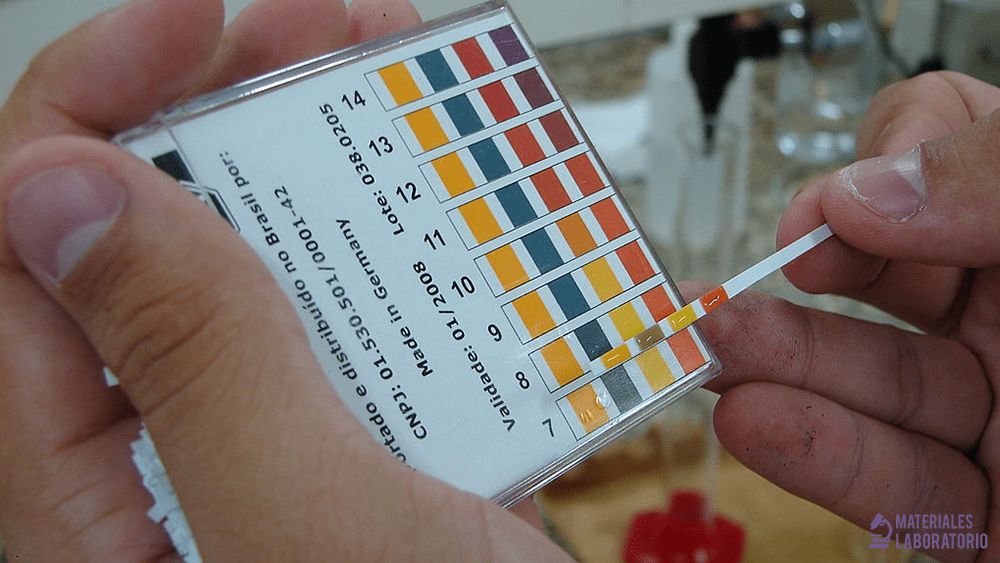
\includegraphics[width=0.8\linewidth]{Imagenes/cap2/Papel-tornasol-min.png}\\
        \caption {Papel tornasol o papel pH. }
        \textbf{Fuente:} Web del fabricante, \cite{noauthor_papel-tornasol-min-768x432png_nodate}.
        \label{fig:tornasol}
    \end{figure}
    \item Amperometr\'ia: La diferencia en la concentraci\'on de iones de hidr\'ogeno (fuera de la sonda vs. dentro de la sonda) crea una corriente muy pequeña. 
    Esta corriente es proporcional a la concentraci\'on de iones de hidr\'ogeno en el l\'iquido medido, \cite{Atlas_pH}. 
    La ventaja de la amperometría como m\'etodo de medici\'on del pH es que es f\'acil de usar. 
    En mediciones amperim\'etricas de pH generaci\'on de hidr\'ogeno ocurre en un metal noble, cuando se combina con un metal menos noble, se forma una c\'elula galv\'anica de distribuci\'on de energ\'ia. 
    Debido a que se generan iones de hidr\'ogeno, la corriente de la c\'elula depende del valor del pH. 
    Las desventajas de este m\'etodo son que las diferencias en la composici\'on de la muestra crean errores muy grandes en las mediciones de pH y el m\'etodo no puede ofrecer resultados fiables en \'acidos y bases extremadamente concentrados, debido a efectos relacionados con la membrana de cristal. 
    \\
    \begin{figure}[ht]
        \centering
        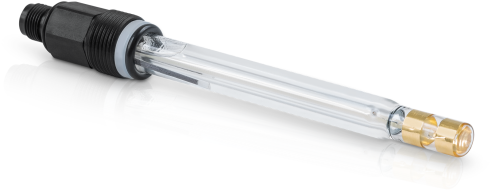
\includegraphics[width=0.8\linewidth]{Imagenes/cap2/amperimetrico.png}
        \caption {Sensor OPTISENS CL 1100.}
        \textbf{Fuente:} Página web del fabricante,
        \cite{ampe_sensores_nodate}.
        \label{fig:amperimetrica}
    \end{figure}

    \item ISFET: \textit{Ion Sensitive Field Effect Transitor} o transistor de efecto campo sensible a iones en un sensor electroqu\'imico que reaccionan a cambios en la actividad de un ion dado, un m\'etodo relativamente nuevo para la medici\'on del valor de pH, \cite{duroux_ion_1991}.
    Es un transistor con fuente de poder y desagüe, dividido por un aislador. 
    Este aislador (puerta) está hecho de un \'oxido met\'alico donde los iones de hidr\'ogeno se acumulan de la misma manera que un electrodo. 
    La carga positiva que se acumula fuera de la puerta se \textit{refleja} en el interior la puerta por una carga negativa igual generada. 
    Una vez que esto sucede, la puerta comienza a conducir electricidad. 
    Cuanto menor sea el valor de pH, m\'as iones de hidr\'ogeno se acumulan y m\'as corriente puede fluir entre la fuente y el drenaje. 
    El ISFET Los sensores, similares a los electrodos de pH de vidrio, act\'uan de acuerdo con la ecuación de Nernst.
    \begin{equation} \label{ecuacion_Nernst} 
        E=E^{0} - \frac{RT}{\eta F}ln(Q)
    \end{equation}
    La ventaja de un ISFET es que es muy peque\~no. 
    La desventaja de usar un ISFET para mediciones de pH es que tienen una durabilidad comparativamente corta y una baja duración a largo plazo, \cite{li_chapter_2019}.
    
    \begin{figure}[ht]
        \centering
        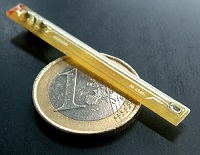
\includegraphics[width=0.8\linewidth]{Imagenes/cap2/ISFET_Euro.jpg}
        \caption {Sensor de pH-ISFET MSFET 3330.} 
        \textbf{Fuente:} Página Web del Fabricante,
        \cite{microsens_nodate}.
        \label{fig:isfet}
    \end{figure}
    
    \item Electrodos: El m\'etodo m\'as com\'un de medic\'on del valor de pH es el uso de electrodos.
    Estos dispositivos de medición de pH son sensores electroqu\'imicos que constan de un electrodo de medici\'on y un electrodo de referencia. 
    El electrodo de medici\'on de pH está hecho de vidrio especial que, debido a sus propiedades superficiales, es particularmente sensible a iones de hidr\'ogeno. 
    El electrodo de medici\'on de pH se llena con una soluci\'on tamp\'on de un valor de pH de 7. 
    Al colocar el electrodo de medici\'on de pH en una prueba soluci\'on, el cambio de voltaje se mide con el electrodo de pH comparando el voltaje medido al electrodo de referencia estable. 
    Este cambio se registra por el medidor de pH y se convierte en el valor de medición de pH que se muestra.
    
\begin{figure}[ht]
    \centering
    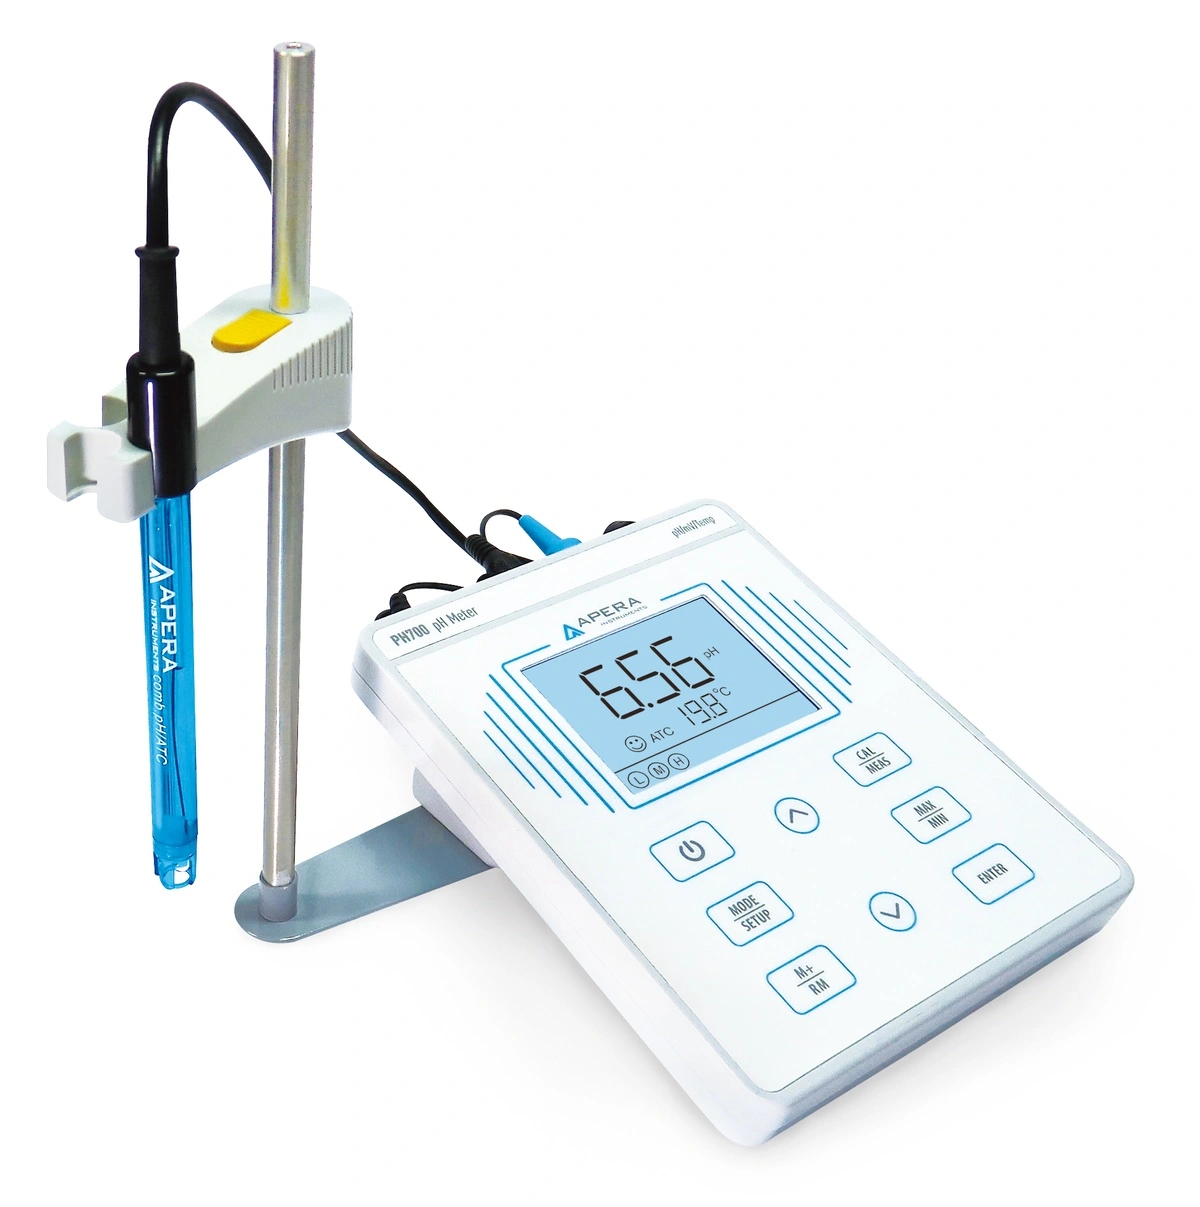
\includegraphics[width=60mm, height=45mm]{Imagenes/cap2/ph700.png}
    \caption {PH700 Benchtop pH Meter Kit. }{\textbf{Fuente:}
    \cite{ph700_nodate} }
    \label{fig:ph700}
    \end{figure}
\end{itemize}

De todos estos métodos de medición del valor de pH,  el mejor es el uso de electrodos de pH. 
No hay otro sistema de medición de pH que proporcione mejor confiabilidad, precisión y velocidad de la medición del pH. 
La desventaja mínima de usar electrodos de vidrio para pH para este m\'etodo de medici\'on de pH es el hecho de que los electrodos de vidrio son delicados y deben manipularse con cuidado, \cite{li_chapter_2019}.

\subsection{Medición de potencial ORP-REDOX}
\subsubsection{¿Que es ORP?}
El potencial de oxidaci\'on-reducci\'on (ORP) se define como la fuerza electromotriz entre un electrodo de metal noble y un electrodo de referencia cuando se sumergen en una soluci\'on.
Los electrodos de ORP son inertes y miden la relaci\'on entre las actividades de las especies oxidadas y las reducidas presentes, \cite{d19_committee_test_nodate}.
Tambi\'en conocido como redox, es una medida en milivoltios y mide el potencial de intercambio de electrones, si una sustancia (generalmente l\'iiquida) se oxida o se reduce. 
Los oxidantes siempre tendrán un valor de ORP positivo, mientras que los reductores siempre tendrán un valor de ORP negativo. 
El ORP se usa com\'unmente para medir la limpieza en los sistemas de agua y la descomposici\'on de productos de desecho, escombros y contaminantes. 
La composici\'on química del agua subterránea y los sistemas de acu\'feros contaminados se ven afectados por procesos de reducción de oxidación (redox), \cite{wator_redox_2020}.

\subsubsection{¿Cómo medirlo?}
Un sensor de ORP consta de un electrodo de ORP y un electrodo de referencia.
Los electrodos de ORP miden de forma fiable el ORP en casi todas las soluciones acuosas y, en general, no están sujetos a la interferencia de la solución por el color, la turbidez, la materia coloidal y la materia en suspensión, \cite{d19_committee_test_nodate}.
El electrodo OPR: el principio detr\'as de la medici\'on de ORP es el uso de un electrodo de metal inerte (platino, a veces oro), debido a su baja resistencia, ceder\'a electrones a un oxidante o aceptar\'a electrones de un reductor. 
El electrodo de ORP continuará aceptando o cediendo electrones hasta que desarrolle un potencial, debido a la carga acumulada, que es igual al ORP de la soluci\'on. 
La precisión t\'ipica de una medida de ORP es d\'e \( \pm5 mV\).
El electrodo de referencia:  ser el mismo electrodo de plata-cloruro de plata utilizado con mediciones de pH, \cite{li_chapter_2019}.

\begin{figure}[ht]
    \centering
    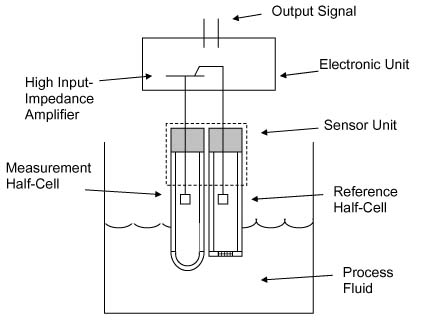
\includegraphics[width=0.8\textwidth]{Imagenes/cap2/ORP_Sensor_Image.jpg}
    \caption {Diagrama del sensor OPR. }
    \textbf{Fuente:} Página web del fabricante,
    \cite{orp_sensor_measure_nodate}.
    \label{fig:opr}
\end{figure}

\subsection{Temperatura}
La temperatura se puede medir utilizando un sensor de temperatura de los diferentes tipos que existen, todos ellos infieren la temperatura al detectar alg\'un cambio en una caracter\'istica f\'isica. 

\subsubsection{¿Qué es temperatura?}
La temperatura es una de las medidas más comunes en la vida diaria. 
En el contexto de calidad de agua, la temperatura puede proveer un indicio de las condiciones de vida para plantas acu\'aticas y animales.  
Las temperaturas templadas se consideran generalmente ben\'eficas para el crecimiento de la poblaci\'on acu\'atica. 
De cualquier forma, despu\'es de cierto punto la temperatura puede tener un efecto contrario, contribuyendo a declinar la diversidad biol\'ogica en cuerpos de agua.

\subsubsection{¿Por qu\'e la medición de temperatura es importante?}
Los organismos acu\'aticos c\'omo los peces y plancton son de agua fr\'ia, as\'i que la temperatura en el agua tiene un impacto directo en la temperatura de su cuerpo. 
Estos organismos tienen rangos de temperatura en los cuales pueden sobrevivir y desarrollarse. 
A medida que la temperatura alcanza el l\'imite superior o su rango para un organismo, la actividad biol\'ogica estar\'a en su tope. 
La actividad disminuir\'a cuando se alcance el punto mínimo del rango. 
Si la temperatura excede el rango aceptable para el organismo, la cantidad disponible de ox\'igeno puede ser demasiado baja para sustentarlos. 
Esto se debe a que el agua caliente tiene un punto de saturaci\'on de ox\'igeno menor al agua fr\'ia. 
Si la temperatura est\'a por debajo del rango aceptable, no hay suficiente actividad para el crecimiento de los organismos. 
La temperatura alta tambi\'en contribuye al crecimiento y floración de algas, \cite{cruzado_campos_aplicacion_2021}.
El oxígeno se consume en la medida que bacterias descompongan estos brotes, lo que reduce la cantidad de oxígeno disuelto disponible.
La temperatura en varios cuerpos de agua se basa en la hora del día y la cantidad de luz solar calentando la superficie.
Las temperaturas aceptables tambi\'en var\'ian dependiendo del tipo de r\'io o corriente de agua que desee monitorear. 
La temperatura tambi\'en puede verse influenciada por el flujo y el cuerpo de agua. 
Si el flujo de agua se incrementa, quiz\'a c\'omo resultado de una fuerte lluvia, se puede esperar que la temperatura disminuya. 
El incremento en la corriente tiene c\'omo efecto reducir la temperatura en el agua.
La poluci\'on por temperatura, tambi\'en conocida c\'omo poluci\'on t\'ermica, puede ser causada por vertimientos de agua calentada en asfalto o concreto. 
Esta tambi\'en puede proceder de efluentes industriales que sean descargados en cuerpos de agua, o agua que sea usada cómo refrigerante en plantas de energ\'ia nuclear. 
Estos efluentes significan que el agua en el que son descargadas incrementar\'a la temperatura general del cuerpo de agua.  
La temperatura también puede asociarse a la turbidez.  
Ya que la cantidad de luz absorbida incrementa a medida que el agua se oscurece, la temperatura también aumentar\'a.

\subsubsection{¿Cómo medir la temperatura?}
Muchos termómetros simples usan un termistor.  
El termistor es un dispositivo semiconductor cuya resistencia varía en función de la temperatura, \cite{asale_termistor_nodate}. 
A medida que la temperatura incrementa, la resistencia disminuye.  
La resistencia medida por el termistor se convierte en un valor que se muestra ya sea en la escala Celsius o Fahrenheit.  
Los sensores termistores son adecuados para rangos de temperatura desde -50$^{o}C$ a  150$^{o}C$.

\subsubsection{Sensor de temperatura (T)}
Existen varios tipos de sensores de temperatura, los cuales se pueden encontrar en el mercado: 
\begin{itemize}
    \item \textit{Termopares}: Un  termopar  es  un  dispositivo  para  la  medición  de  la  temperatura,  basado  en  efectos  termoeléctricos.  Como se puede observar en la figura \ref{fig:Termopar},es  un  circuito   formado   por   dos   conductores   de   metales   diferentes  o  aleaciones  de  metales  diferentes,  unidos  en  sus extremos y entre cuyas uniones existe una diferencia de temperatura, que origina una fuerza electromotriz, \cite{rodriguez_medicion_2007}. 
    El principio de funcionamiento de los sensores es efecto Peltier y efecto Thompson. El  efecto  Thompson,  se  caracteriza  por  la  absorci\'on  o  liberaci\'on de calor por parte de un conductor sometido a un  gradiente  de  temperatura,  por  el  que  circula  una  corriente.    Se  libera  calor  cuando  la  corriente  circula  del  punto m\'as caliente hacia el m\'as fr\'io, \cite{logvinov_principios_2007}.
    
    \begin{figure}[ht]
        \centering
        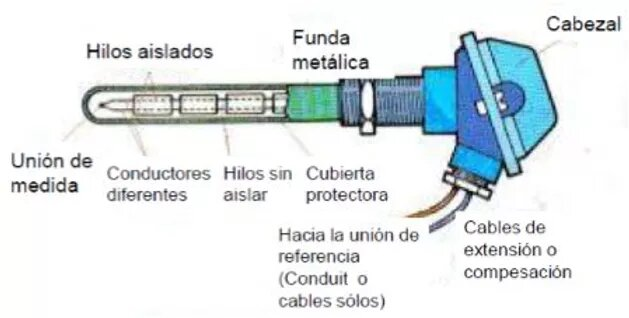
\includegraphics[width=0.8\textwidth]{Imagenes/cap2/termopar.jpg}
        \bigskip
        \caption{Elementos constructivos de un termipar}  \textbf{Fuente:} P\'agina web del fabricante, \cite{universidad_de_carabobo_-termopares_nodate}.
        \label{fig:Termopar}
    \end{figure}
    Los termopares están disponibles en diferentes combinaciones de metales o calibraciones para adaptarse a diferentes aplicaciones. Los tres más comunes son las calibraciones tipo J, K y T, de los cuales el termopar tipo K es el más popular debido a su amplio rango de temperaturas y bajo costo, \cite{omega_termopar_nodate}.
    \item \textit{Dispositivos de temperatura resistivos}: Este    grupo    lo    constituyen    las    RTD    (\textit{Resistance    Temperature  Detector})  y  los  term\'istores.  Las  RTD  son  sensores basados en elementos conductores, mientras que los termistores se fundamentan en semiconductores.
    Al calentarse un metal habrá una mayor agitación térmica, dispersándose más los electrones y reduciéndose su velocidad media, aumentando la resistencia. A mayor temperatura, mayor agitación, y mayor resistencia.
    La variación de la resistencia puede ser expresada de manera matem\'atica:
    \begin{equation} \label{ecuacion_dilatacion} 
        R=R_{o}. (1+\alpha.\Delta T])
    \end{equation}
    Por lo general, la variación es bastante lineal en márgenes amplios de temperatura. Los  dispositivos  RTD  m\'is  comunes  est\'an  construidos  con  una  resistencia  de  platino  (Pt, figura \ref{fig:RTD},  llamadas  tambi\'en  PRTD, aunque tambi\'en se utilizan otros materiales.  T\'ipicamente  tienen  una  resistencia  entre  20 $\Omega$  y  20 $k\Omega$  La  ventaja  más  importante   es   que   son   lineales   dentro   del   rango   de   temperatura entre –200$^{o}C$ y 850$^{o}C$, \cite{rodriguez_medicion_2007}.
    
    \begin{figure}[ht]
        \centering
        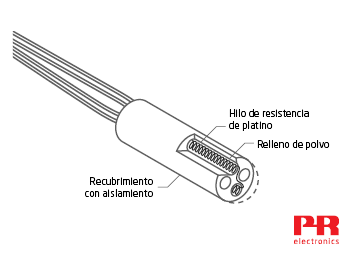
\includegraphics[width=0.8\textwidth]{Imagenes/cap2/RTF.png}\\
        \bigskip
        \caption {RTD de elemento en espiral}
        \textbf{Fuente:} P\'agina web del fabricante, \cite{prelectronics_fundamentos_nodate}.
        \label{fig:RTD}
    \end{figure}
    % [RR] 15MAYO2022
    \item \textit{Radiadores infrarrojos}: consiste en una lente para enfocar los rayos infrarrojos (IR) de energía a un pirómetro, que convierte la energía en una señal eléctrica que se puede mostrar en unidades de temperatura después de ser compensada por la variación de la temperatura ambiente \ref{fig:radiante}. Esta configuración facilita la medición de temperatura sin contacto con el objeto a medir.
    Como tal, el term\'ometro de infrarrojos es útil para medir la temperatura en circunstancias donde termopares, sondas Pt100 u otros sensores de temperatura por contacto no pueden ser utilizados o no producen datos exactos por una variedad de razones, \cite{omega_termometro_nodate}.
    
    \begin{figure}[ht]
        \centering
        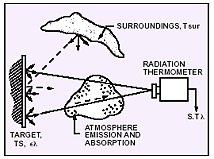
\includegraphics[width=0.8\textwidth]{Imagenes/cap2/radiante.jpg}
        \bigskip
        \caption {Medici\'on de temperatura por radiaci\'on infraroja}  
        \textbf{Fuente:} P\'agina web del fabricante, \cite{omega_como_nodate}.
        \label{fig:radiante}
    \end{figure}
    
    \item \textit{Dispositivos bimet\'alicos}:  La temperatura se puede medir de muchas maneras, basándose en la dilatación, termómetros bimetálicos, efecto Seebeck, \cite{martinez_soriano_evaluacion_2020}, que consiste en la de producción de electricidad a partir del contacto entre dos metales diferentes, dos semiconductores, o un metal y un semiconductor, que se hallen en un mismo circuito, debido a la diferencia de temperatura entre ellos, \cite{universidad_publica_de_navarra_introduccion_nodate}. 
    Tal como se parec\'ia en la figura \ref{fig:biMetal}, consiste en dos metales t\'ermicamente diferentes pegados uno contra otro. Cuando disminuye la temperatura, los contactos tienden a se cierran y dan paso a la corriente el\'ectrica que pasa a trav\'es del termostato. Cuando se eleva la temperatura, un metal tiende a expandirse  m\'as que el otro y la tira bimet\'alica unida se dobla hacia arriba (o hacia abajo), lo que abre los contactos y evita que la corriente fluya.
    
    \begin{figure}[ht]
        \centering
        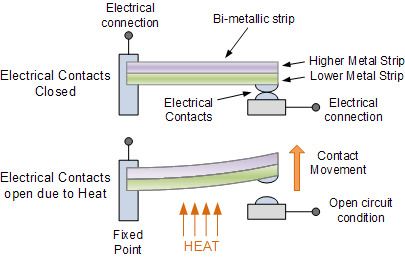
\includegraphics[width=0.8\textwidth]{Imagenes/cap2/biMetal.jpg}\\
        \bigskip
        % \raggedright
        \caption { termostato bimet\'alicol } 
        \textbf{Fuente:} P\'agina web del fabricante, \cite{huseyn_a_sensores_2020}.
        \label{fig:biMetal}
    \end{figure}
    
    \item \textit{Dispositivos de dilatación de l\'iquido}: Los dispositivos de dilatación de fluido, en general, vienen en dos clasificaciones principales observadas en la figura \ref{fig:dilatacion_li}: el tipo de mercurio y el tipo de líquido orgánico. También hay disponibles versiones que usan gas en lugar de líquido. El mercurio se considera un riesgo ambiental, así que hay regulaciones que rigen el embarque de dispositivos que lo contienen. Los sensores de dilatación de fluido no requieren energía eléctrica, no plantean riesgos de explosión y son estables incluso después de ciclos repetidos. Por otra parte, no generan datos que se registren o transmitan fácilmente, y no pueden hacer mediciones puntuales,\cite{omega_engineering_inc_medicion_nodate}.
    
    \begin{figure}[ht]
        \centering
        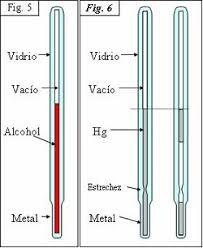
\includegraphics[width=0.8\linewidth]{Imagenes/cap2/Dilatacion Liquida.jpg}\\
        \bigskip
        % \raggedright
        \caption { Term\'ometros de dilataci\'on l\'iquida  } \textbf{Fuente}. Extra\'ido de web, \cite{equipos_y_laboratorio_de_colombia_termometros_nodate}.
        \label{fig:dilatacion_li}
    \end{figure}
\end{itemize}

\subsection{Conductividad (CE) / Total de sólidos disueltos (TDS)}
\subsubsection{¿Qué es la conductividad?}
La conductividad eléctrica (CE) mide que tan bien una sustancia puede transmitir una corriente eléctrica. 
Pequeñas partículas cargadas, llamadas iones, pueden ayudar a transportar la corriente eléctrica a través de la substancia. 
Estos iones pueden estar cargados positiva, o negativamente. A mayor cantidad de iones disponibles, mayor será la conductividad; menores iones resultarán en una menor conductividad. 
La CE se reporta de manera habitual en miliSimens por centímetro (mS/cm).
El total de sólidos disueltos (TDS) es la cantidad de sustancias disueltas en soluciones. Las mediciones permiten conocer las sustancias orgánicas e inorgánicas disueltas en el líquido. 
Los resultados de esta lectura se muestran en miligramos por litro (mg/L), partes por mill\'on (ppm), gramos por litro (g/L), o partes por mil (ppt).

\subsubsection{¿Por qu\'e la medici\'on de conductividad es importante?}
La conductividad eléctrica (CE) es otra manera de evaluar la calidad del agua, ya que al incrementar la presencia de total de sólidos disueltos (TDS), expresada en la CE, puede ser un indicador de contaminantes. 
La CE puede verse afectada por los carbonatos presentes en el agua caliza, contaminantes humanos como aguas residuales u otro tipo de fuente cómo sistemas de pozos sépticos o residuos de agricultura.
Altas concentraciones de TDS pueden reducir la calidad de agua y causar problemas en el balance de agua para organismos individuales. 
Por otra parte, bajas concentraciones pueden limitar el crecimiento de vida acuática. 
Algunos de los efectos comentados para parámetros como el dióxido de carbono y acidez tienen relevancia para la CE, cómo su impacto negativo en la fotosíntesis. 
Esto se debe a que al incrementar la cantidad de sólidos el agua se oscurecerá, reduciendo la tasa de fotosíntesis. 
La CE proveerá un indicio del total de sólidos disueltos, del cual el total de sales disueltas es un componente. 
Si el nivel de sales en el TDS es alto, esto también puede contribuir a acidificar el agua. 
De cualquier forma, si el nivel de carbonatos en la lectura de TDS son altos, esto podría contribuir a incrementar la alcalinidad, lo que puede ayudar a proteger el agua ante cambios ácidos. 
Esta es una buena respuesta de interrelación, entre los parámetros de calidad de agua.
Adem\'as es importante comprender que es importante comprender la relación entre TDS y sólidos totales. Los sólidos totales se refieren a toda la materia sólida, ya sea suspendida o disuelta en agua. 
Los sólidos disueltos no son visibles en el agua, ya que al disolverse se vuelven parte de la solución. 
Los TDS son una medida de las sustancias disueltas en agua que están en una muestra de agua. 
En una muestra recolectada en un r\'io, estas sustancias disueltas se conocen cómo solutos, y el agua es llamada solvente.

\subsubsection{¿Cómo medir la conductividad?}
La mejor manera de medir la conductividad es con el uso de un medidor. 
Dos electrodos que aplican un voltaje AC se ubican en la solución. 
Esto crea una corriente que depende de la conductividad natural de la solución. 
El medidor lee esta corriente y muestra la conductividad (CE) o ppm (TDS)

\subsubsection{Sensor de conductividad eléctrica (CE) }
La salinidad de un suelo o agua, se refiere a la cantidad de sales presentes en solución, y puede ser estimada indirectamente mediante la medición de la conductividad eléctrica (CE). 
El valor de CE es influenciado por la concentración y composición de las sales disueltas.
A mayor valor de CE, mayor es la salinidad presente. 
Es importante considerar que todos los fertilizantes inorgánicos son sales y por lo mismo tienen un efecto directo sobre la CE.
La salinidad es un fenómeno indeseable, ya que afecta el crecimiento de las plantas de varias maneras y por lo mismo, un aumento en la CE traerá como consecuencia una disminución de rendimiento, \cite{rebolledo_v_conductividad_2017}.

\subsection{Oxígeno disuelto (OD)}
\subsubsection{¿Qué es el oxígeno disuelto?}
La concentración de oxígeno disuelto (OD) en agua es extremadamente importante en la naturaleza, al igual que para los ambientes artificiales. 
En océanos, lagos, ríos, y otros grandes cuerpos de agua, el oxígeno disuelto es esencial para el crecimiento y desarrollo de la vida acuática. 
Sin oxígeno, el agua puede volverse tóxica debido al decaimiento de la materia orgánica por bacterias anaeróbicas. 
En un ambiente industrial, el agua debe contener al menos 2 mg/L de oxígeno para proteger a las tuberías de corrosión.  

\subsubsection{¿Por qu\'e es importante el oxígeno disuelto?}
Los niveles de OD pueden ayudar a indicar la salud de un cuerpo de agua. 
Si los niveles de OD están dentro de la media o más altos, el agua es un buen ambiente para una amplia variedad de vida acuática. 
Si los niveles de OD son bajos, indica la presencia de contaminantes en el agua. 
Algunas especies de vida acuática pueden subsistir en agua con un amplio rango de OD; pero otras fallecen a bajos niveles de OD.
Se espera que las lecturas de OD tengan una amplia fluctuación si la fuente de agua cuenta con abundante vida vegetal. Esto se debe al proceso de fotosíntesis, \cite{hannacolombia_guipara_nodate}. 
Ya que existe una menor actividad fotosintética en las noches, cuando la luz no está presente, y que tanto plantas como animales seguirán consumiendo oxígeno a través de la respiración, los niveles de OD en las horas de la mañana serán mucho menores a los de otras horas del día. 
Una vez inicia la fotosíntesis, los niveles de OD incrementarán. 
Este es un buen ejemplo de los beneficios de medir los parámetros varias veces durante el día. 
Si únicamente se realiza la medición de OD antes del amanecer, se llegará a una conclusión inadecuada sin importar la salud del cuerpo de agua.
Mientras que los niveles de OD se influencian particularmente por la actividad fotosintética, una gran cantidad de OD se obtiene de la mezcla del OD y el agua. 
Esto sucede si el agua es turbulenta en grandes cuerpos de agua. 
La turbulencia incrementa el área superficial del agua, para que el oxígeno atmosférico puede mezclarse más fácilmente. 
El aire tiene una concentración de oxígeno que es 20 veces mayor que la concentración de ox\'igeno en el agua. 
La diferencia de concentración resulta en el oxígeno atmosférico disolviéndose en agua cuando las dos se encuentran. 
Si hay más superficie de agua en su interfaz, entonces más oxígeno del aire se absorberá.
Otros factores que influencian los niveles de OD son la temperatura y los vertimientos. 
El ox\'igeno se disuelve más f\'acilmente en agua fría, y el agua fría tiene la capacidad de mantener mayores cantidades de gas que el agua tibia, así que el nivel de OD disuelto disminuye a medida que el agua se calienta.
Los vertimientos pueden incluir desechos orgánicos o contaminantes creados por el hombre; en ambos casos, los organismos en el agua deben usar oxígeno en el proceso de descomponer estos contaminantes.  
También, los desechos orgánicos pueden llevar al crecimiento de vegetación acuática.  
Cuando las plantas mueren al final del lapso de crecimiento, grandes cantidades de oxígeno disuelto se consumen al descomponerse.

\subsubsection{¿Cómo podemos medir el oxígeno disuelto?}
Las concentraciones de ox\'igeno disuelto se reporta en miligramos  por litro de agua, mg/L. (La unidad equivalente a mg/L es equivalente a partes por millón=ppm)  
Las lecturas de OD se realizan habitualmente utilizando una sonda y un medidor.
Es importante realizar lecturas de OD en varios momentos del día, y a varias profundidades. 
Las mediciones le darán una visión general de los niveles de OD en el cuerpo de agua que investiga. 
Cómo sucede con todos los parámetros de calidad de agua, este parámetro debe monitorearse en el tiempo. 
Esto producirá suficiente información para identificar y evaluar tendencias.

\subsubsection{Sensor de ox\'igeno disuelto (DO):}
Toda la vida acuática depende de la disponibilidad de oxígeno disuelto (DO) en el agua. 
Mientras que los organismos terrestres viven en una atmósfera compuesta aproximadamente de un 20\% de ox\'igeno, los organismos acuáticos sobreviven con una cantidad de ox\'igeno considerablemente menor. 
La solubilidad del ox\'igeno en agua dulce var\'ia entre 14.6 mg/L a 0$^{\circ}$C hasta aproximadamente 7 mg/L a 35$^{\circ}$C bajo una presión de 760 mmHg. La concentración de oxígeno disuelto en agua está determinada por la ley de Henry, que describe la relación de equilibrio entre la presión parcial de oxígeno atmosférico y la concentración de oxígeno en agua. 
Otros factores que influyen la concentración de oxígeno disuelto en agua son: la presión atmosférica (y, por lo tanto, la altitud sobre el nivel del mar), el contenido de sales en el agua, y la temperatura del agua. 
El contenido de ox\'igeno disuelto en cuerpos de agua puede disminuir significativamente por efecto de la respiración, especialmente la microbiana, resultante de la degradación de compuestos orgánicos. 
Traducido eso a un sensor cu\'al permita detectar estos factores, se tiene la sonda galvánica de ox\'igeno disuelto que consta de una membrana de politetrafluoroetileno (PTFE), un ánodo bañado en un electrolito y un cátodo. 
Las mol\'eculas de oxígeno se desactivan a través de la membrana de la sonda a una velocidad constante (sin la membrana, la reacción es rápida). 
Una vez \'el las mol\'eculas de ox\'igeno han atravesado la membrana, se reducen en el c\'atodo y se produce una pequeña tensión. 
Si no hay moléculas de ox\'igeno presentes, la sonda emitir\'a 0 mV. 
A medida que aumenta el ox\'igeno, tambi\'en lo hace la salida de mV de la sonda. La sonda emite un voltaje diferente en presencia de ox\'igeno. Lo \'unico que es constante es que 0mV = 0 ox\'igeno.